\documentclass[border=3pt]{standalone}
% Shared preamble for every generated figure.
% Matches the report: newtx (Times), greyscale, square boxes.
\usepackage{newtxtext,newtxmath}
% newtx's typewriter (txtt) draws a slashed zero; use Latin Modern instead.
\renewcommand{\ttdefault}{lmtt}
\usepackage{tikz}
\usetikzlibrary{positioning,arrows.meta,calc,fit,backgrounds,shapes.geometric,
                decorations.pathreplacing,decorations.pathmorphing,matrix,patterns}

\definecolor{figgrey}{gray}{0.88}
\definecolor{figmid}{gray}{0.60}
\definecolor{figdark}{gray}{0.35}

\tikzset{
  fig/.style={font=\small},
  box/.style={draw,thick,minimum height=8mm,minimum width=22mm,align=center,
              inner sep=2pt,font=\small},
  greybox/.style={box,fill=figgrey},
  smallbox/.style={draw,minimum height=6mm,minimum width=16mm,align=center,
                   inner sep=2pt,font=\scriptsize},
  ln/.style={-{Stealth[length=2.2mm,width=1.8mm]},thick},
  lnb/.style={{Stealth[length=2.2mm,width=1.8mm]}-{Stealth[length=2.2mm,width=1.8mm]},thick},
  lbl/.style={font=\scriptsize,inner sep=1.5pt},
  note/.style={font=\scriptsize\itshape,inner sep=1.5pt},
}

\newcommand{\ins}[2]{\makebox[16mm][l]{\ttfamily #1}\makebox[30mm][l]{\ttfamily #2}}
\newcommand{\elt}[2]{\makebox[16mm][l]{#1}\makebox[19mm][l]{\ttfamily #2}}
\begin{document}
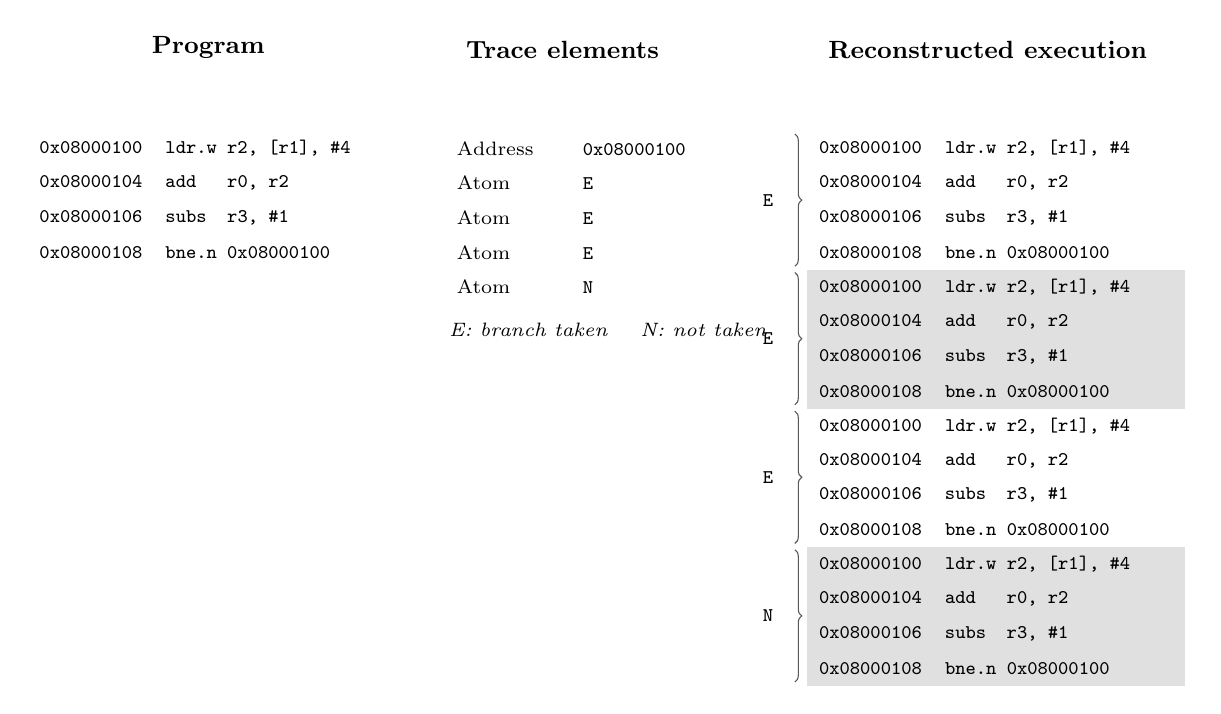
\begin{tikzpicture}[fig,
  hdr/.style={font=\small\bfseries,anchor=south},
  row/.style={anchor=north west,minimum height=4.4mm,font=\scriptsize,inner xsep=1.5mm},
  band/.style={fill=figgrey}]

\def\rh{4.4}
\def\xB{5.3}
\def\xC{9.9}

% ------------------------------------------------ 1: the program
\node[hdr] at (2.3,0.35) {Program};
\foreach \a/\t [count=\n from 1] in {%
  0x08000100/{ldr.w r2, [r1], \#4}, 0x08000104/{add\ \ \ r0, r2},
  0x08000106/{subs\ \ r3, \#1},      0x08000108/{bne.n\ 0x08000100}}
  {\node[row] at (0,-\n*\rh mm) {\ins{\a}{\t}};}

% ------------------------------------------------ 2: the element stream
\node[hdr] at (\xB+1.5,0.35) {Trace elements};
\foreach \k/\v [count=\n from 1] in {%
  Address/0x08000100, Atom/E, Atom/E, Atom/E, Atom/N}
  {\node[row] at (\xB,-\n*\rh mm) {\elt{\k}{\v}};}
\node[note,anchor=north west] at (\xB,-6.4*\rh mm)
     {E: branch taken\ \ \ \ N: not taken};

% ------------------------------------------------ 3: the reconstruction
\node[hdr] at (\xC+2.3,0.35) {Reconstructed execution};
\foreach \i in {1,3}{
  \pgfmathsetmacro{\yb}{-(1+4*\i)*\rh}
  \node[band,anchor=north west,minimum width=48mm,minimum height=17.6mm]
    at (\xC,\yb mm) {};
}
% brace tying each atom to the block of instructions it implies
\foreach \n/\atom in {0/E,1/E,2/E,3/N}{
  \pgfmathsetmacro{\yt}{-(1+4*\n)*\rh}
  \pgfmathsetmacro{\yv}{-(5+4*\n)*\rh}
  \draw[decorate,decoration={brace,amplitude=2.5pt},figdark]
    ($(\xC,\yt mm)+(-1.5mm,-0.4mm)$) -- ($(\xC,\yv mm)+(-1.5mm,0.4mm)$);
  \pgfmathsetmacro{\ym}{(\yt+\yv)/2}
  \node[font=\scriptsize\ttfamily,anchor=east]
    at ($(\xC,\ym mm)+(-3mm,0)$) {\atom};
}

\foreach \n in {0,1,2,3}{
  \pgfmathsetmacro{\ya}{-(1+4*\n)*\rh}
  \pgfmathsetmacro{\yc}{-(2+4*\n)*\rh}
  \pgfmathsetmacro{\yd}{-(3+4*\n)*\rh}
  \pgfmathsetmacro{\ye}{-(4+4*\n)*\rh}
  \node[row] at (\xC,\ya mm) {\ins{0x08000100}{ldr.w r2, [r1], \#4}};
  \node[row] at (\xC,\yc mm) {\ins{0x08000104}{add\ \ \ r0, r2}};
  \node[row] at (\xC,\yd mm) {\ins{0x08000106}{subs\ \ r3, \#1}};
  \node[row] at (\xC,\ye mm) {\ins{0x08000108}{bne.n\ 0x08000100}};
}

\end{tikzpicture}
\end{document}
